\documentclass[10pt]{beamer}

%%%
% PREAMBLE FOR THIS DOC 
%%%
%https://tex.stackexchange.com/questions/68821/is-it-possible-to-create-a-latex-preamble-header
\usepackage{/Users/miw267/Repos/latex_preamble/beamer_preamble}


%%%
% AGENDA TOPICS
%%%
\agendatopic[intuition]{Partitions: the intuition}
\agendatopic[from-equiv]{From equivalence relations to partitions}
\agendatopic[from-partitions]{From partitions to equivalence relations}
\agendatopic[count]{Using equivalence relations to count}


%%%
% DOCUMENT
%%%

\begin{document}

%\maketitle

%% Title page frame
%\begin{frame}
%    \titlepage 
%\end{frame}





\title{09/28/2025: Partitions}
\author{CSCI 246: Discrete Structures}
\date{Textbook reference: Sec 16, Scheinerman}

\begin{frame}
    \titlepage 
\end{frame}


\begin{frame}
%\begin{mygreenbox}[title=Graded Quiz Pickup]
%Quizzes are in the front of the room, grouped into four bins (A-G, H-L, M-R, S-Z) by last name. The quizzes are upside down with your last name on the back. Come find yours before, during, or after class.  Only turn the quiz over if it's yours.
%\end{mygreenbox} 
%\vfill 

%\begin{myredbox}[title=Announcements]
%
%\begin{itemize}
%\item Please write your name on the attendance form. 
%\item Paul has changed his office hours to Mon, Wed 3-4pm in Barnard 259	.
%\item Reminder: Solutions to group exercises are included in the slides posted everyday after class (by 6pm).
%\end{itemize}
%
%
%
%\end{myredbox}
%
%\vfill 


\begin{myyellowbox}[title=Today's Agenda]
\begin{itemize}
	\item Review early course feedback ($\approx$ 10 mins)
	\item Mini-lecture ($\approx$ 25 mins)
	\item Group exercises ($\approx$ 15 mins)
\end{itemize}

%	Rationale for group exercises: we got shortchanged on time last couple days, and I already did a lot of lectures, so I want you to practice. Next problems quiz will cover relations and functions: Hamkins and 
%	
\end{myyellowbox}
\vfill 

\end{frame}


\begin{frame}[standout]

Early course feedback
	
\end{frame}



\begin{frame}{Review of early course feedback}

\begin{itemize}
	\item Most people want more time for group exercises.  \pause \alert{I'll make sure to protect time for this on Monday and Wednesday. If you have ideas about Friday, please share.} \pause  
	\item Don't want to get punished for getting proof question on Quiz 2 correct.  \pause \alert{This was made extra credit.} \pause  \alert{\underline{Note: All scores went up or stayed the same!}} \pause 
	\item Post whiteboard pictures to repo. \pause \greencheck \pause 
	\item Can we do the same groups for one week? \pause \alert{Let's take a poll on how people feel about this.}
	\item Want homework.  \pause \alert{Let's take a poll to disentangle how much is a grade buffer and how much is wanting earlier feedback.} \pause \alert{I'll post an follow-up announcement after class.}
	\item Quizzes are mis-graded. \pause \alert{Feel free to bring them to me for review/re-grading.} \pause  \alert{Let's look at one example question.} \pause 
\end{itemize}
\end{frame}

%%%%%%%%%%%%%%%%%
\agendaframe{intuition}


\begin{frame}
\small 
\colorbox{yellow!30}{\textbf{Demo.}} Stand by the whiteboard that best characterizes you: do you have 0 siblings, 1 sibling, or 2 or more siblings?
\pause 
\vfill
\colorbox{blue!30}{\textbf{Notion.}} A mathematical \textbf{partition} means breaking a whole thing into non-overlapping pieces so that every single item belongs to one and only one piece, with nothing left out and nothing shared twice.
We've just partitioned the class!
\pause 
\vfill 
\colorbox{green!30}{\textbf{Example.}} We just \textbf{partitioned} the class in terms of number of siblings: 0, 1, or $2^+$.
\pause 
\vfill 

\begin{mygreenbox}[title=Definition]
Let $A$ be a set.  A \textbf{partition} of $A$ is a set of non-empty, pairwise disjoint sets whose union is A. \only<2->{\alert{(Recall: Disjoint sets have no elements in common.)}}
\end{mygreenbox}

\pause 
\vfill 
\colorbox{green!30}{\textbf{Example (continued).}} Let $A$ be the students, TA, and teacher for the class.  We've formed the partition $A= A_0 \cup A_1 \cup A_{2+}$ where individuals in $A_i$ have $i$ siblings:
\begin{align*}
A_0 &= \set{???, \hdots} \\
A_1 &= \set{\text{Mike W.}, \text{Madhav}, \hdots} \\
A_{2+} &= \set{???, \hdots} \\	
\end{align*}


\end{frame}



\begin{frame}{Partitions in everyday life}
\small 

\newcommand{\figtables}{%
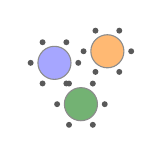
\begin{tikzpicture}[scale=0.42]
  \foreach \cx/\cy/\c in {0/0/blue!35, 1.6/0.35/orange!55, 0.8/-1.25/green!45!black!55}{
     \begin{scope}[shift={(\cx,\cy)}]
       \draw[black!45, fill=\c] (0,0) circle (0.5);
       \foreach \a in {0,60,...,300}{\fill[black!65] (\a:0.72) circle (0.09);}
     \end{scope}}
\end{tikzpicture}}

\begin{tabular}{@{}p{0.72\textwidth}@{\hspace{0.6em}}c@{}}
\textbf{Sorting laundry.} Whites, darks, colors.  Every item goes in one basket,
no item is in two, and nothing is left on the floor.
& \raisebox{-0.5\height}{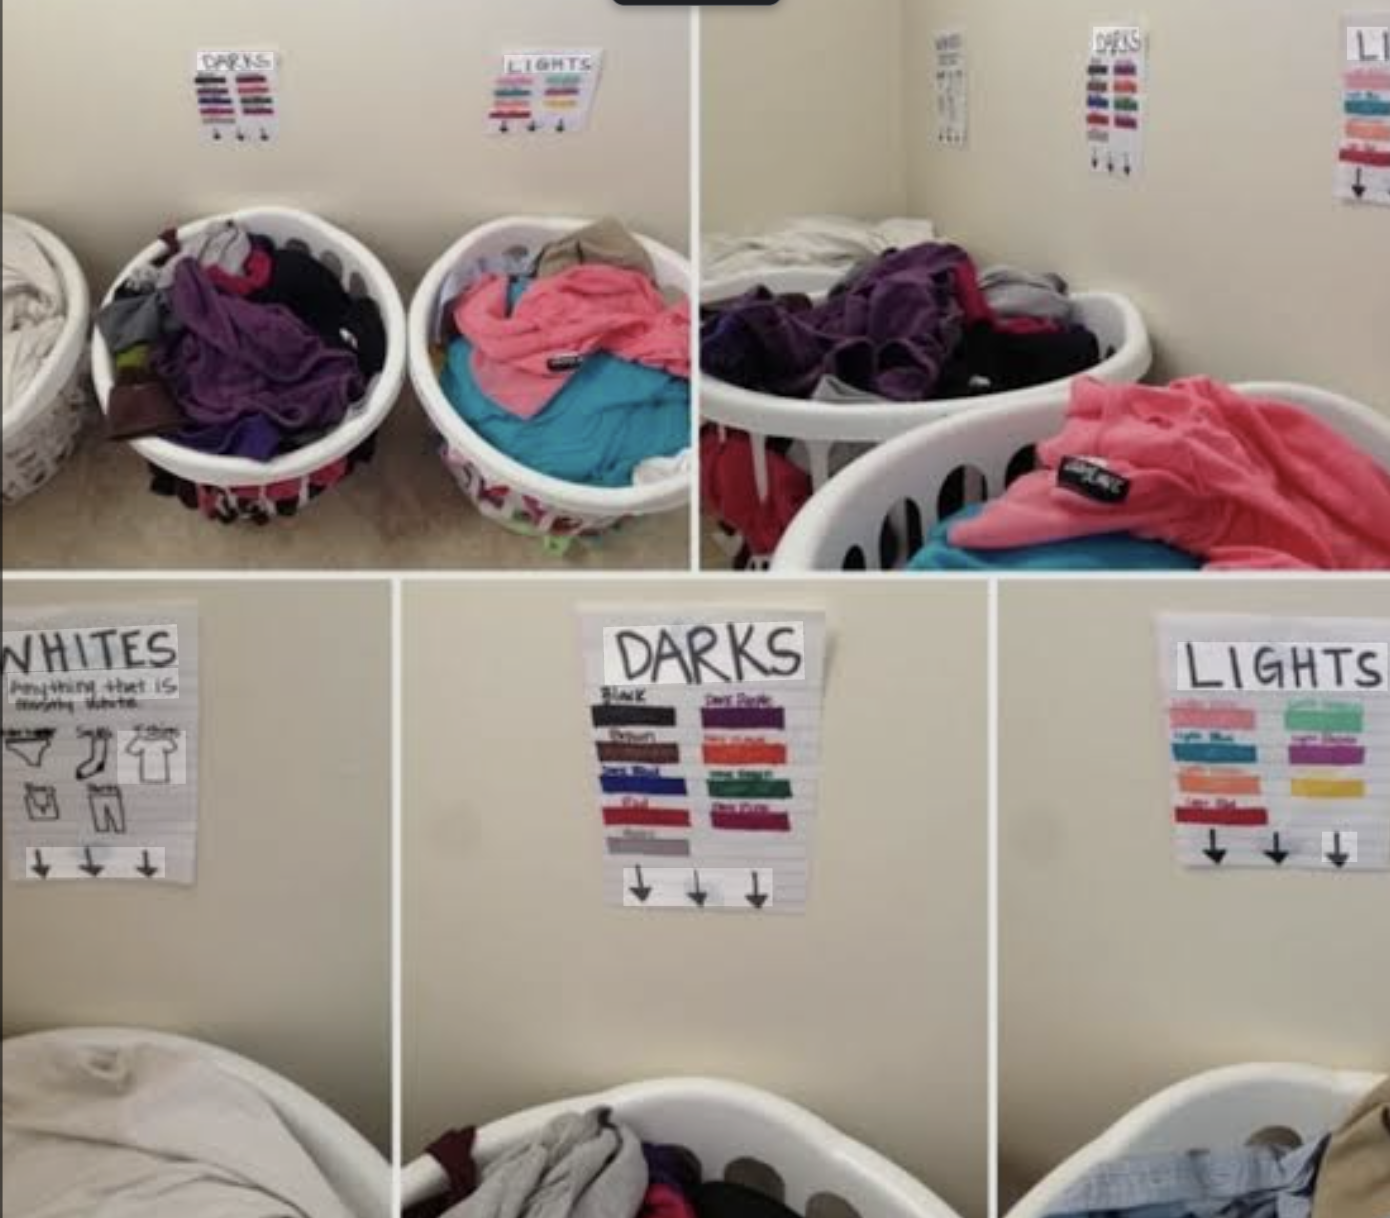
\includegraphics[height=1.5cm]{images/laundry}} \\[0.7em]
\pause
\textbf{A calendar.} A year splits into 12 months, a week into 7 days.  Every hour
of your life belongs to exactly one day.
& \raisebox{-0.5\height}{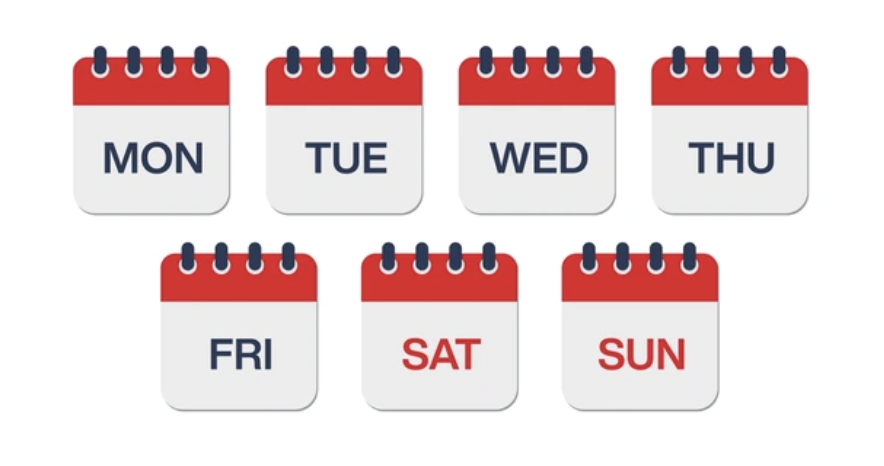
\includegraphics[height=1.5cm]{images/week}} \\[0.7em]
\pause
\textbf{A jigsaw puzzle.} Each piece covers its own patch of the picture. Together
they cover all of it, with no overlap.
& \raisebox{-0.5\height}{
\includegraphics[height=1.5cm]{images/jigsaw}} \\[0.7em]
\pause
\textbf{A wedding seating chart.} Every guest sits at exactly one table, and nobody
is split between two.
& \raisebox{-0.5\height}{\figtables} \\
\end{tabular}
\pause 
\vfill \vfill 
\colorbox{yellow!30}{\textbf{Poll.}} Any other examples?
\end{frame}

\begin{frame}{Partition failures}

\colorbox{yellow!30}{\textbf{Another demo.}}  Stand by the whiteboard that best characterizes you: do you have a dog or a cat? 

\vfill
\pause
	
\colorbox{red!30}{\textbf{Assessment.}} This demo breaks! Someone has both, someone has neither (or a goldfish).  We can't form a partition of the class this way. 
\end{frame}

%%%%%%%%%%%%%%%%%
\agendaframe{from-equiv}


\begin{frame}{From equivalence relations to partitions}
\small 
\colorbox{yellow!30}{\textbf{Poll.}} Is the following an equivalence relation on the set $A=\{1,2,3,4,5,6\}$?
%
\begin{align*}
R &=\{ (1,1), (1,2), (2,1), (2,2), (3,3), \\
& \quad (4,4), (4,5), (4,6), (5,4), (5,5), (5,6), (6,4), (6,5), (6,6)	\}
\end{align*}

\vfill 
\pause 
\colorbox{green!30}{\textbf{Solution.}} We need to check:
\begin{itemize}
\item \textit{Reflexivity}: Does $xRx$ for all $x \in A$? \pause \greencheck 
\item \textit{Symmetry}:  Does $xRy$ imply $yRx$ for all $x,y \in A$?  \pause \greencheck  
\item \textit{Transitivity}:  \pause  Does $xRy$ and $yRz$ imply $xRz$ for all $x,y,z \in A$?   \pause \greencheck 
\end{itemize}
\end{frame}



\begin{frame}{From equivalence relations to partitions}
\colorbox{yellow!30}{\textbf{Poll.}} Since $R$ below is an equivalence relation, we can form the equivalence classes of $R$.  What are they?
%
\begin{align*}
R &=\{ (1,1), (1,2), (2,1), (2,2), (3,3), \\
& \quad (4,4), (4,5), (4,6), (5,4), (5,5), (5,6), (6,4), (6,5), (6,6)	\}
\end{align*}

\vfill 
	

\only<2->{\colorbox{green!30}{\textbf{Solution.}}}

\begin{columns}

\begin{column}{0.5\textwidth}
\begin{align*}
\only<2->{[1] &= [2] = \set{1,2} \\} 
\only<2->{[3] &= \set{3} \\} 
\only<2->{[4] &= [5] = [6] = \set{4,5,6}}	
\end{align*}
\end{column}
\pause 
\only<2->{
\begin{column}{0.45\textwidth}
\begin{center}
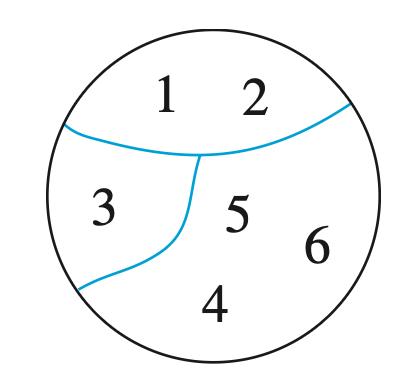
\includegraphics[width=.7\textwidth]{images/equiv_classes.png}	
\end{center}
\end{column}
}
\end{columns}

\only<3->{\colorbox{red!30}{\textbf{Reminder.}} The notation $[a]$ is the equivalence class associated with $a$.}
\end{frame}




\begin{frame}{From equivalence relations to partitions}
\small

\begin{mygreenbox}[title=Definition]
Let $A$ be a set.  A \textbf{partition} of $A$ is a set of non-empty, pairwise disjoint sets whose union is A. \only<2->{\alert{(Recall: Disjoint sets have no elements in common.)}}
\end{mygreenbox}

\vfill
\only<3->{\colorbox{green!30}{\textbf{Example.}} The diagram below provides a partition of $A=\set{1,2,3,4,5,6}$.
\begin{center}
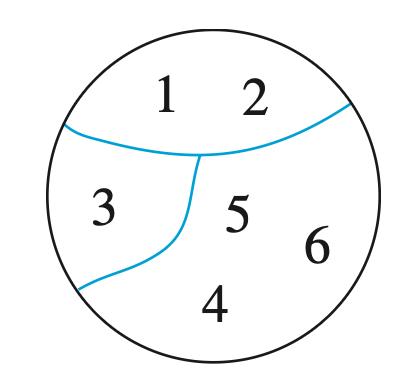
\includegraphics[width=.2\textwidth]{images/equiv_classes.png}
\end{center}
In this case, the partition has 3 \textit{parts} (or \textit{cells}).}
\vfill
\only<4->{\colorbox{yellow!30}{\textbf{Poll.}} How do we know it's a partition?}
\only<5->{Let's check the definition.}
\only<5->{\begin{itemize}
\item Are the parts disjoint? \only<6->{\greencheck  \scripttext{[Recall (from Def 12.6) that two sets are \textbf{disjoint} if they have no elements in common.]}}
\item Does the union of the parts equal $A$? \only<7->{\greencheck}
\end{itemize}}

\end{frame}

\begin{frame}{From equivalence relations to partitions: The general case}


\colorbox{blue!30}{\textbf{Let's summarize.}} So far, we've shown that the relation $R$ below is an \alert{equivalence relation} on the set $A=\set{1,2,3,4,5,6}$: 
%
\begin{align*}
R &=\{ (1,1), (1,2), (2,1), (2,2), (3,3), \\
& \quad (4,4), (4,5), (4,6), (5,4), (5,5), (5,6), (6,4), (6,5), (6,6)	\}
\end{align*}
%
\vfill 
\pause 
So the relation $R$ makes \alert{equivalence classes}: 
%
\begin{columns}
\begin{column}{0.5\textwidth}
\begin{align*}
[1] &= [2] = \set{1,2} \\
[3] &= \set{3} \\
[4] &= [5] = [6] = \set{4,5,6}	
\end{align*}
\end{column}
\pause 
\begin{column}{0.45\textwidth}
\begin{center}
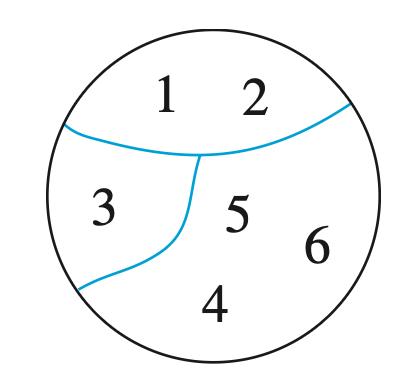
\includegraphics[width=.4\textwidth]{images/equiv_classes.png}	
\end{center}
\end{column}
\end{columns}
%
\vfill 
\pause 
By definition, these equivalence classes form a \alert{partition} of $A$.

\pause 
\vfill 

This phenomenon is true \alert{generally}.

\begin{mygreenbox}[title=\text{Cor. 15.13 Scheinerman (restated on pp. 85)}]

Let $R$ be an equivalence relation on a set $A$.  The equivalence classes of $R$ form a partition on the set $A$.
\end{mygreenbox}
	
\end{frame}


%
%\begin{frame}[standout]
%Below this still needs to be absorbed.
%	
%\end{frame}



%\begin{frame}
% \begin{myredbox}[title=Reading Quiz (Partitions)]  
%\begin{enumerate}
%	\item Give an example of a partition of the set $\set{1,2,3,4,5,6}$.
%	\item How many different ways are there to rearrange the letters in the word \texttt{AARDVARK}?
%\end{enumerate}
%\end{myredbox}
%\vfill 
%\begin{mygreenbox}[title=Problems Quiz (Relations)]
%\begin{enumerate}
%\item The property \textit{irreflexive} is not the same as being not reflexive.  Give an example of a relation on a set that is neither reflexive nor irreflexive.   (You may express your answer either as a set of ordered pairs or as a graph.) 
%\item A relation $R$ is defined on $\mathbb{Z}$ by $a\,R\,b$ if $a+b$ is even.  Is $R$ an equivalence relation? If so, pick one of the 3 properties that all equivalence relations have and prove that $R$ has that property.  If not, prove that $R$ is not an equivalence relation. 	
%\end{enumerate}
%
%\end{mygreenbox}
%\vfill 
%%\textbf{Remark.} For intuition, note that $x \equiv y$ (mod $n$) if $x$ and $y$ have the same remainder after dividing by $n$.  For example, $6 \equiv 1$ (mod 5).
%\end{frame}



%\begin{frame}{Partitions}
%
%\begin{mygreenbox}[title=Definition]
%Let $A$ be a set.  A \textbf{partition of} $A$ is a set of nonempty, pairwise disjoint sets whose union is $A$	
%\end{mygreenbox}
%\vfill 
%\begin{myredbox}[title=Example]
%Let $A = \set{1,2,3,4,5,6}$, and let
%\[ \mathcal{P} = \bigg\{ \set{1,2}, \set{3}, \set{4,5,6} \bigg\} \]	
%
%\vfill
%\begin{figure}
%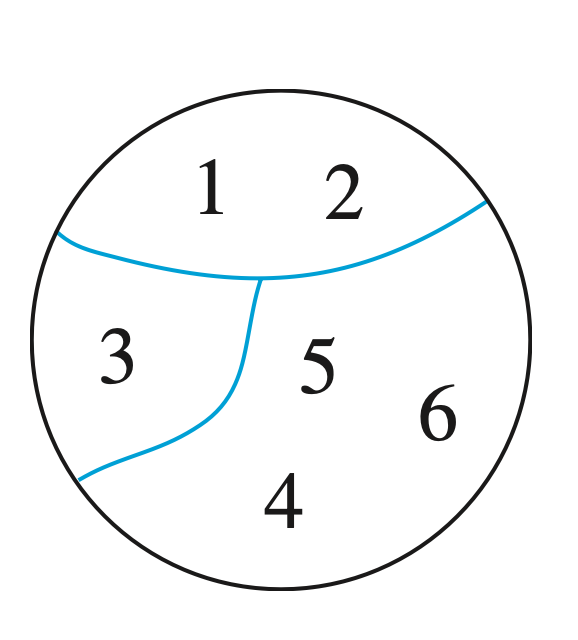
\includegraphics[width=0.2\textwidth]{images/partition.png}	
%\end{figure}
%\end{myredbox}
%
%\end{frame}

\begin{frame}{From equivalence relations to partitions: Another example}
\small 
 \begin{mygreenbox}[title=\text{Proposition (Scheinerman pp. 85)}]  
Let $R$ be an equivalence relation on $A$.  The equivalence classes of $R$ form a partition of the set $A$. 
\end{mygreenbox}
\vfill 
\begin{myredbox}[title=Example]
Let's set $R$ to congruence mod 3.  We've shown $R$ is an equivalence relation. Thus, we can partition $A= \set{\text{the integers}}$ into the following equivalence classes
%
\begin{align*}
[0] &= \set{\hdots, -6, -3, 0, 3, 6, \hdots} \\	
[1] &= \set{\hdots, -5, -2, 1, 4, 7, \hdots} \\	
[2] &= \set{\hdots, -4, -1, 2, 5, 8, \hdots}
\end{align*}
\end{myredbox}
\vfill
\pause 
\colorbox{blue!30}{\textbf{Reminder.}} How do we know it's a partition? \pause  Let's check the definition.
\begin{itemize}
\item Are the parts disjoint? \pause \greencheck  \scripttext{[They have no elements in common.]}
\item Does the union of the parts equal $A$? \pause \greencheck 
\end{itemize}


\end{frame}


%%%%% OUTLINE
\agendaframe{from-partitions}


\begin{frame}{From partitions to equivalence relations}
\footnotesize 

\begin{myredbox}[title=Example]

\begin{minipage}{0.2\textwidth}

\begin{figure}
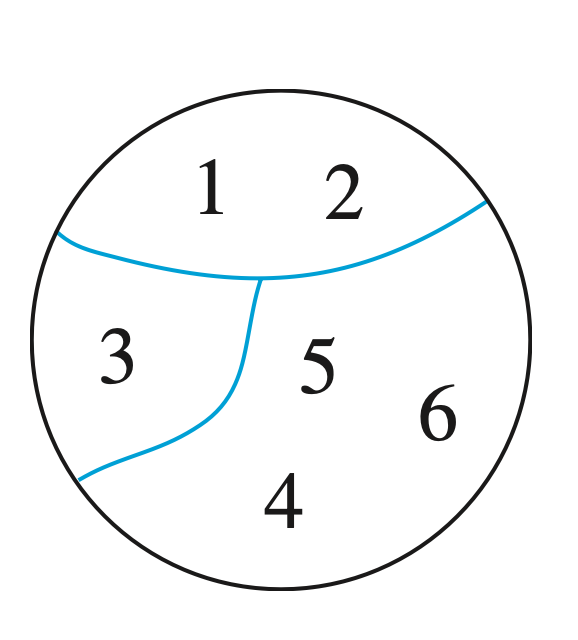
\includegraphics[width=0.7\textwidth]{images/partition.png}	
\end{figure}
\end{minipage}
\hfill 
\begin{minipage}{0.73\textwidth}
Starting from the partition on the left, we can reconstruct the equivalence relation:
%
\begin{align*}
R &=\{ (1,1), (1,2), (2,1), (2,2), (3,3), \\
& \quad (4,4), (4,5), (4,6), (5,4), (5,5), (5,6), (6,4), (6,5), (6,6)	\}
\end{align*}
\end{minipage}
\end{myredbox}
\vfill 
\pause 
 \begin{mygreenbox}[title=Definition]  
Let $\mathcal{P}$ be a partition on a set $A$. The \textbf{is-in-the-same-part-as} relation, denoted  $\stackrel{\mathcal{P}}{=}$, is given by
\[ a \stackrel{\mathcal{P}}{=} b \quad  \iff \quad \exists P \in \mathcal{P} : a,b \in P \]
\end{mygreenbox}
\vfill 
 \begin{mygreenbox}[title=\text{Proposition (Scheinerman Prop 16.3)}]  
Let $\mathcal{P}$ be a partition on a set $A$. The relation $\stackrel{\mathcal{P}}{=}$ is an equivalence relation on $A$.
\end{mygreenbox}
\vfill 
\pause 
\begin{myyellowbox}[title=Remark]
In gist, we can take elements in the same cell to be related to each other. 
\end{myyellowbox}


\end{frame}



%%%%% OUTLINE
\agendaframe{count}


\begin{frame}{Using equivalence relations to count}
\footnotesize 
 \begin{myyellowbox}[title=Question]  
How many ways are there to rearrange the letters in the word \texttt{HELLO}?
\end{myyellowbox}
\vfill 
\pause 
 \begin{myredbox}[title=Solution]  
If there were no repeated letters (imagine a big and small L), the answer would be $5!=120$.
%
\begin{figure}
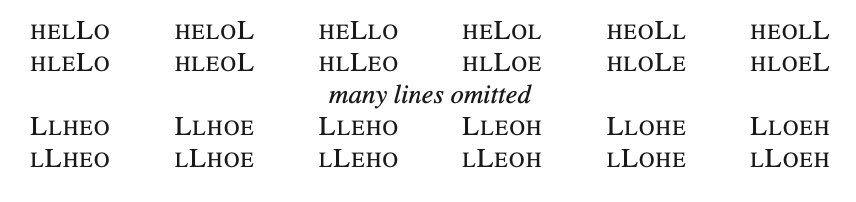
\includegraphics[width=0.9\textwidth]{images/hello}	
\end{figure}
%
\pause 
But we want to treat the big and small $L$ as equivalent.  So we form equivalence classes, each of which have 2 members.
%
\begin{figure}
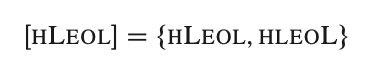
\includegraphics[width=0.5\textwidth]{images/hello_equiv}	
\end{figure}
%
\pause 
All together there are $\frac{120}{2} = 60$ equivalence classes.  Hence, the answer is 60.
\end{myredbox}

\end{frame}

\begin{frame}
 \begin{mygreenbox}[title=\text{Theorem: Counting Equivalence Classes (Scheinerman Thm 16.6)}]  
Let $R$ be an equivalence relation on a finite set $A$. If all the equivalence classes of $R$ have the same size, $m$, then the number of equivalence classes is $|A|/m$. 
\end{mygreenbox}

\vfill 
\pause 
\colorbox{blue!30}{\textbf{Remark.}} You'll practice applying this theorem during the group exercises.
\end{frame}



\end{document}
